
\documentclass[a4paper,twoside]{report}
\usepackage{INScore}
\usepackage{pslatex}
\usepackage[T1]{fontenc}
\usepackage[utf8]{inputenc}
\usepackage{graphicx}
\usepackage{amssymb}
\usepackage{rail}
\usepackage{makeidx}
\usepackage{color}
\usepackage{hyperref}
\usepackage{comment}
\usepackage{multicol}
\usepackage{textcomp}

\definecolor{mycolor}{rgb}{0.384,0.0,0.145}
\hypersetup{
	colorlinks=true,
	linkcolor= mycolor
}


\setlength\parskip{\medskipamount}

\makeatletter
\railparam{\addtolength{\itemsep}{-3ex}}

%\newcommand{\toplevel}[1]	{\section{#1}}
%\newcommand{\sublevel}[1]	{\subsection{#1}}
%\newcommand{\subsublevel}[1]	{\subsubsection{#1}}

\newcommand{\toplevel}[1]	{\chapter{#1}}
\newcommand{\sublevel}[1]	{\section{#1}}
\newcommand{\subsublevel}[1]	{\subsection{#1}}

\newcommand{\fullref}[1]	{\ref{#1} p.\pageref{#1}}

\providecommand{\boldsymbol}[1]{\mbox{\boldmath $#1$}}
\newcommand{\OSC}[1]		{\texttt{#1}}
\newcommand{\values}[1]		{\texttt{#1}}
\newcommand{\oldexample}	{\hspace*{1cm}}
\newcommand{\example}		{\textbf{\hspace{-1.5cm}\textbf{\textsc{Example }}}}
\newcommand{\note}	[1]		{\vspace{2mm}\textbf{\hspace{-1.03cm}\textbf{\textsc{Note #1}}}}
\renewcommand{\seealso}		{\textbf{See also: }}

\newcommand{\osctype}[1]	{\textbf{\texttt{{\small #1}}}}
\newcommand{\oscint}		{\osctype{int32}}
\newcommand{\oscfloat}		{\osctype{float32}}
\newcommand{\oscstring}		{\osctype{string}}
\newcommand{\rational}		{\osctype{rational}}

\newcommand{\lowTilde} 		{\texttildelow}

\let\olditemize\itemize
\let\oldenditemize\enditemize
\renewenvironment{itemize} 	{\olditemize \setlength{\itemsep}{1mm}}{\oldenditemize}


\setlength\parskip{2pt}
\setlength\railnamesep{-1mm}
\railterm{int32, float32, string}
\railalias{int32}{\oscint}
\railalias{float32}{\oscfloat}
\railalias{string}{\oscstring}


\definecolor{mygrey}{gray}{0.93}
\newcommand{\sample}	[1]			{\vspace{-2mm}\begin{center}\colorbox{mygrey}{
								\begin{minipage}[t]{0.9\columnwidth} 
								{\small \texttt{#1}}
								\end{minipage}}\end{center}}
\newcommand{\samplev}[1]			{\begin{center}\colorbox{mygrey}{
								\begin{minipage}[t]{\columnwidth} 
								{\small \texttt{#1}}
								\end{minipage}}\end{center}}
\newcommand{\sampleindent}	{ \hspace{0.5cm} }

\newcommand{\warning}[1]	{\textbf{\textsc{Warning:}} #1}

\makeatother
\makeindex


\begin{document}

\title{INScore \\ Evaluable Expression Reference \\v.0.1}

\author{D. Fober\\ GRAME\\ Centre national de cr\'eation musicale\\
{\small <fober@grame.fr>} \\
%\vspace{2mm}
%ANR-08-CORD-010
}

\maketitle


\tableofcontents

\pagestyle{plain}

\newpage

\setcounter{page}{1}

%===============================
%:General format
\toplevel{Score expressions}
\label{scoreExpr}

\emph{Score expressions} allows to defines score objects (\OSC{gmn} or \OSC{pianoroll}) by dynamically combine various resources using a formal expression. To define such object one should use the basic \OSC{set} messages using a score expressions as arguments:

\example\\
The following example defines a \OSC{gmn} and a \OSC{pianoroll} object using score expressions, the meaning of the expression is explained further.
\sample{/ITL/scene/score set gmn expr(seq [a] [b]); \\
/ITL/scene/pianoroll set pianoroll expr(score);}

%===============================
\sublevel{General Syntax}

A score expression  always starts with \OSC{expr(} and ends with \OSC{)}, then 
2 syntaxes are handled:

\begin{rail}
EvaluableExpression: 	('expr')
						'('
						 (
						  ([1] operator score score)
						  |[2] score
						 )
						')'
\end{rail}

\begin{itemize}
\item \textbf{1}: Define an expression as an operation combining two scores. \OSC{operator} is the name of the operation used to combine them (see Section~\ref{operators} for operators list), and \OSC{score} are the arguments passed to  the operator (see Section~\ref{arguments} for arguments specification).
\item \textbf{2}: Define on expression using a single score. This syntax is useful when defining an object as a dynamic copy of an other existing object or file.
\end{itemize}
Each of these tokens can, of course, be separated by spaces, tabulations or carriage returns (allowing multiline expression definition).

When defining an object using a score expressions, INScore will parse it, construct an internal representation and finally evaluate it, reducing the formal expressions to a valid GMN string.

\example \\
Creating a guido object by sequencing two guido string
\sample{
/ITL/scene/score set gmn expr( seq "[c d e]" "[f g h]");
}
is equivalent to
\sample{
/ITL/scene/score set gmn "[c d e f g h]";
}

\sublevel{Score Operators}
\label{operators}
All the score operators of INScore make use of guido operators implemented in the GuidoAR library.
\begin{table*}[htdp]
\begin{center}
\begin{tabular}{rll}
\hline
operation & arguments		&	description \\
\hline
seq 	&	$s1\ s2$		& puts the scores $s1$ and $s2$ in sequence \\
par 	&	$s1\ s2$		& puts the scores $s1$ and $s2$ in parallel \\ 
rpar	&	$s1\ s2$		& puts the scores $s1$ and $s2$ in parallel, right aligned \\
top 	&	$s1\ s2$ 	& takes as many voices as $s2$ contains from $s1$, starting by the top voice \\
bottom 	&	$s1\ s2$ 	& takes as many voices as $s2$ contains from $s1$, starting by the bottom voice  \\
head	& 	$s1\ s2$	& takes the head of $s1$ up to $s2$ duration \\
evhead 	&	$s1\ s2$	& id. but on events basis i.e. the cut point is specified by $s2$ events count \\
tail	&	$s1\ s2$ 	& takes the tail of a $s1$ after the duration of $s2$ \\
evtail 	&	$s1\ s2$ 	& id. but on events basis i.e. the cut point is specified by $s2$ events count \\
transpose 	&	$s1\ s2$	& transposes $s1$ so its first note of its first voice match $s2$ one \\
duration 	&	$s1\ s2$	& stretches $s1$ to the duration of $s2$  \\
			& 	& if not used carefully, this operator can output impossible to display rhythm\\
pitch 	&	$s1\ s2$	& applies the pitches of $s1$ to $s2$ in a loop \\
rhythm 	&	$s1\ s2$	& applies the rhythm of $s1$ to $s2$ in a loop \\
\hline
\end{tabular}
\end{center}

\end{table*}

%===============================
\sublevel{Score Arguments}
\label{arguments}
The syntax for arguments is quite permissive and various resources can be used as arguments for score expressions. In any case, when evaluating the expression, all the arguments will be reduce to GMN string so they can then be processed by the operators.
\begin{rail}
Argument: 	 GmnCode
			|(	
				( | '\&' | '$\sim$' )
				(		
					 filepath
					|ScoreObject
				)
			 )
			| 	EvaluableExpression
\end{rail}

\subsubsection{Arguments specification}

\begin{itemize}
\item \OSC{GmnCode} are not evaluated, passed as they are to operators. Both GMN and MusicXML string are supported.
\item \OSC{filepath}: on evaluation INScore read all the content of the file. Again, both GMN and MusicXML are supported. \OSC{filepath} handle absolute or relative path (from the scene rootPath) as well as url.
\item \OSC{ScoreObject}: Gmn code can be retreive from existing score objects (\OSC{gmn} or \OSC{pianoroll}) simply refering to them using their identifier (using absolute or relative path).
\item \OSC{EvaluableExpression}: an expression can also be used as an argument, thus simple operator can be combined together to create more complex ones. In that case the \OSC{expr} token can be omitted: parenthesis are sufficient.
\end{itemize}

\subsubsection{Arguments prefix}

\begin{itemize}
\item \OSC{\&}: When triggering the reevaluation of an expression (see Section~\ref{exprCmd}) only the arguments prefixed with \OSC{\&} are updated.


\item \OSC{\lowTilde}: before the first evaluation of a score expression, any \OSC{ScoreObjects} prefixed with a \OSC{\lowTilde} shall be replaced by their own expression. In other words, score expressions containing \OSC{\lowTilde} arguments will be expended with existing score expressions. This mechanism allows to compose not only scores and score expressions together.

\end{itemize}

\example\\
Defining \OSC{/ITL/scene/score} as a copy of \OSC{/ITL/scene/simpleScore} duplicated 4 times.
\sample{/ITL/scene/simpleScore set gmn "[e \{c,g\} |]";\\
\\
/ITL/scene/score set gmn expr( \&simpleScore );\\
/ITL/scene/score set gmn expr( seq \lowTilde score \lowTilde score);\\
/ITL/scene/score set gmn expr( par \lowTilde score \lowTilde score);\\
}
\OSC{/ITL/scene/score} should look like:\\
\begin{center}
 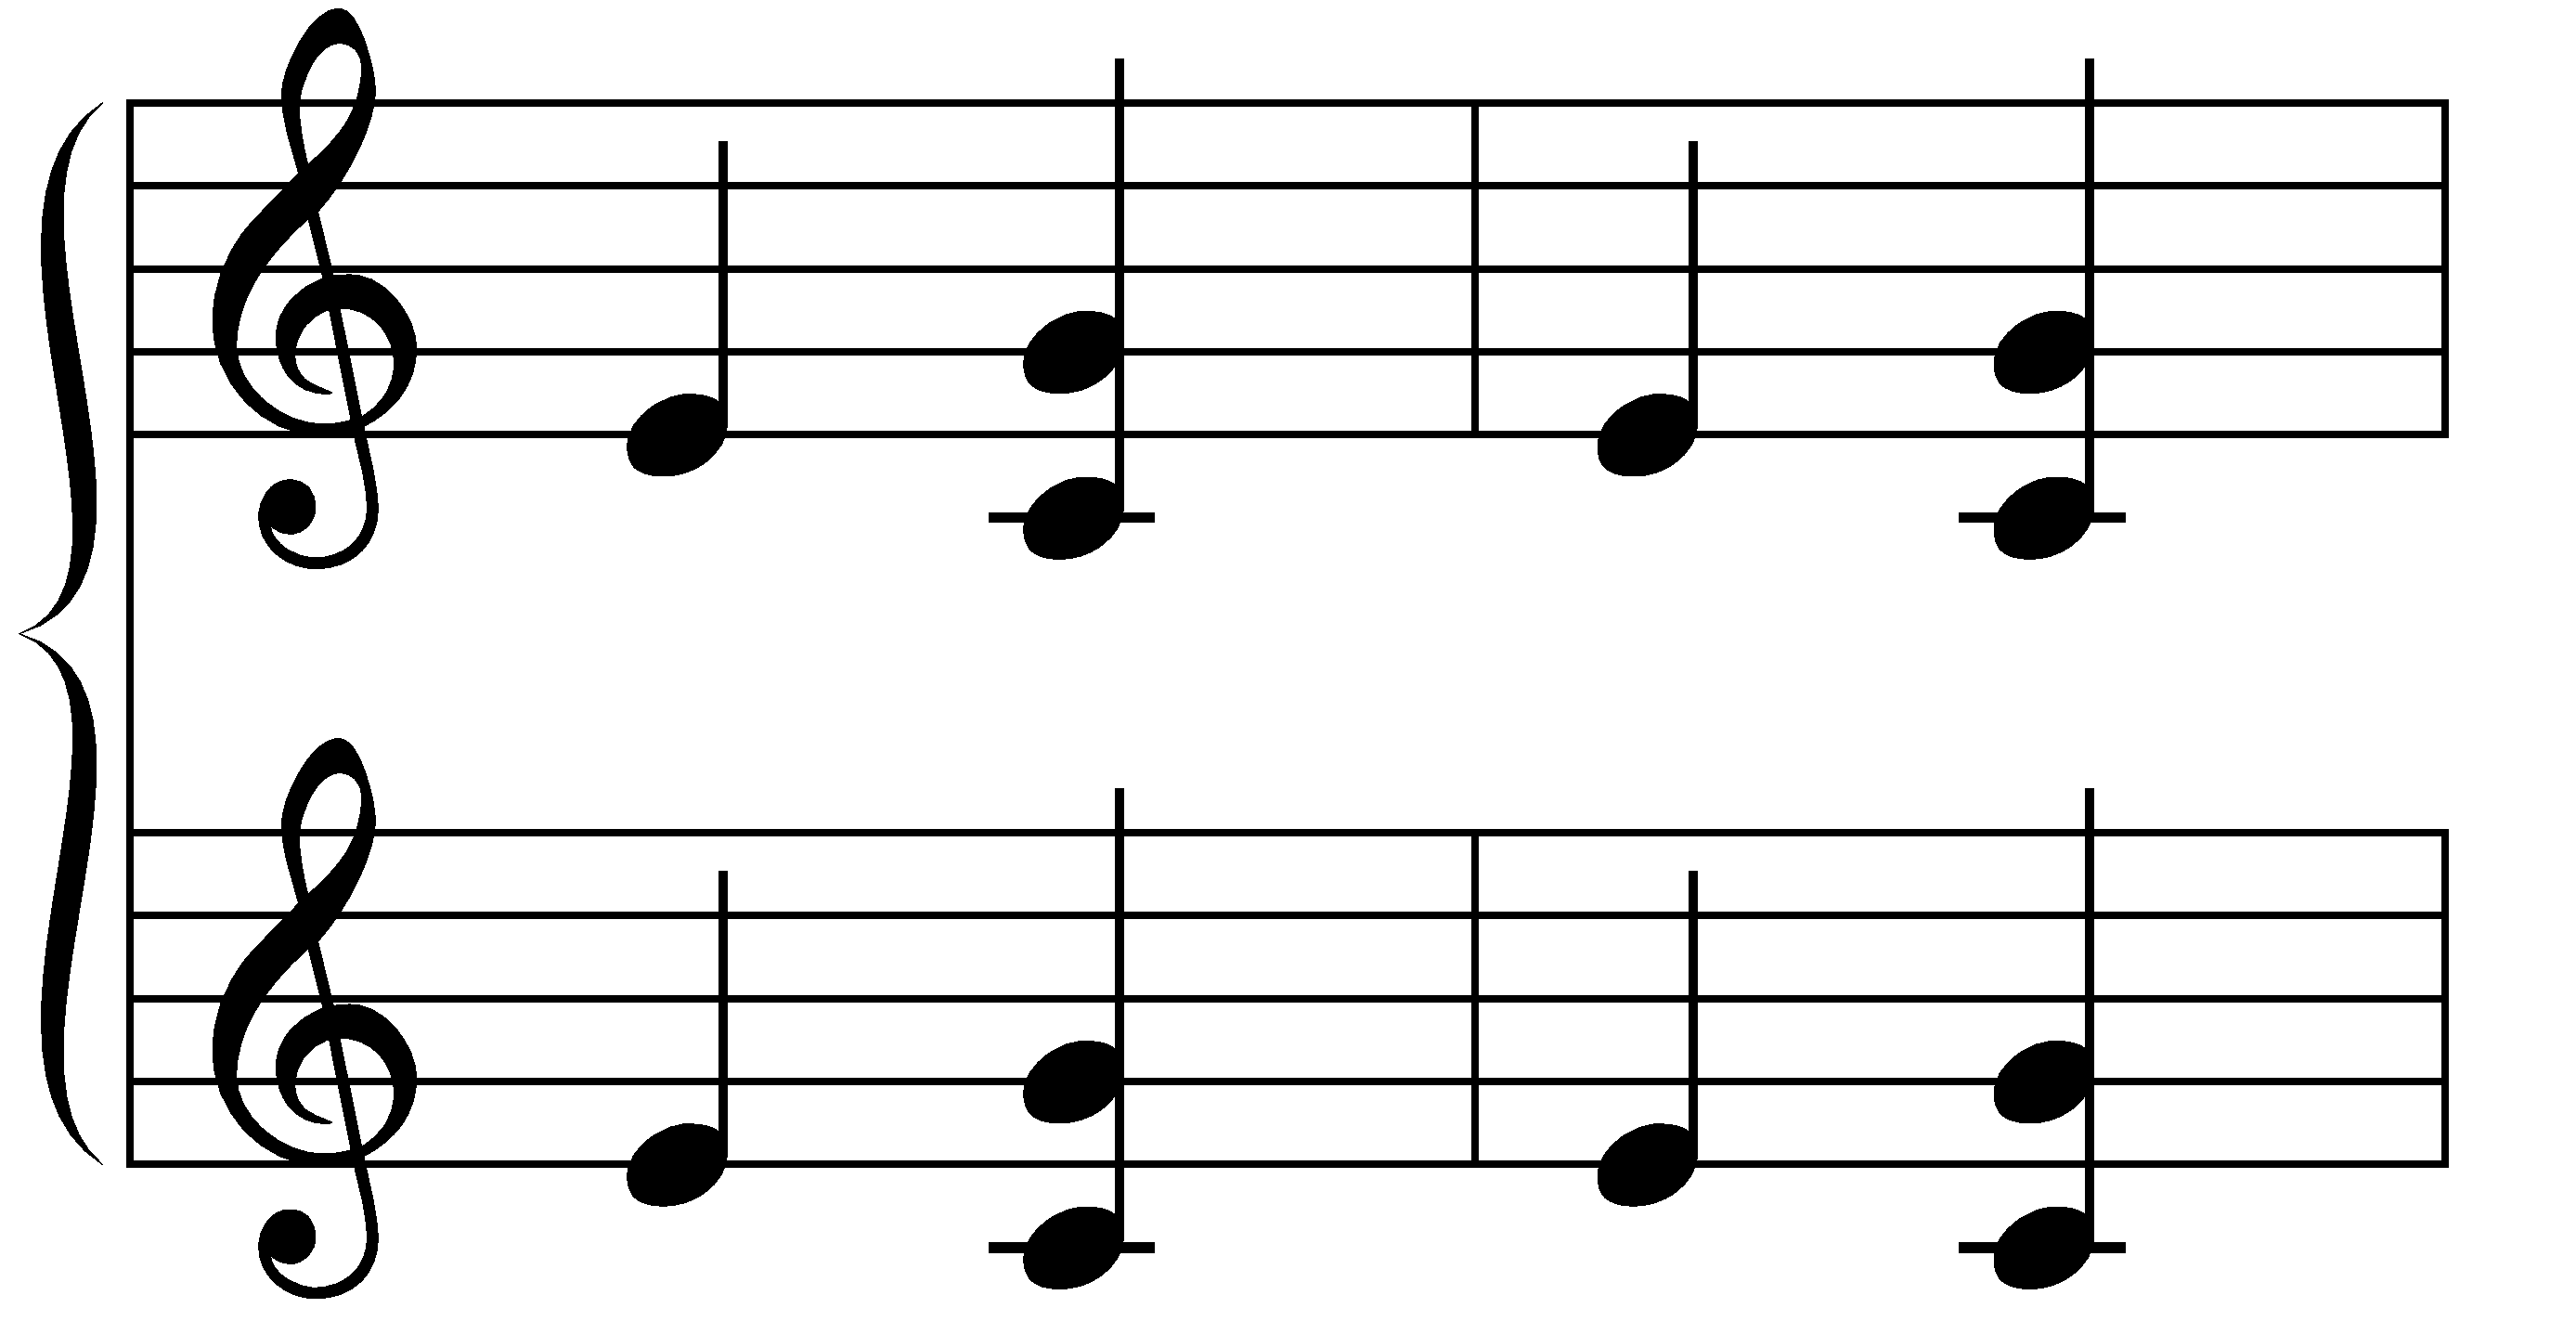
\includegraphics[scale=0.1]{imgs/seqparEnhanced}
\end{center}

Asking for the expanded expression of \OSC{/ITL/scene/score} (see Section~\ref{exprCmd}) should return:

\begin{verbatim}
/ITL/scene/score expr
expr( par
       ( seq
          &simpleScore
          &simpleScore
       )
       ( seq
          &simpleScore
          &simpleScore
       )
    )
\end{verbatim}
\smallbreak


\note {on arguments quoting} \\
Arguments using special characters (space, tabulation, parenthesis, braces...), should be simple or double quoted, otherwise quotes can be omitted.


\pagebreak

%===============================
\sublevel{\OSC{expr} commands}
\label{exprCmd}

ITLObject defined using an evaluable expression gain access to these specific commands:

\begin{itemize}
\item \OSC{get expr}: return the expression used to define the object (before the expansion of \OSC{\lowTilde} arguments).
\item \OSC{get exprTree}: return the expanded expression

\item \OSC{expr reeval}: re-evaluate the expression, updating only the value of arguments prefixed with \OSC{\&}.
\item \OSC{expr reset}: re-evaluate the expression, updating the value of all arguments.
\item \OSC{expr renew}: reapply the definition of the object (similar to send its \OSC{set} message again)
\end{itemize}

Applied to an object which wasn't defined by an evaluable expression, all this commands will cause a bad argument error.
\smallbreak

The \OSC{renew} command reset the internal state of the evaluated variable, forcing the re-evaluation and update of every arguments in the expression. Be aware that the track of copy evaluated arguments is lost after the first evaluation, thus renewing an expression defined using copy evaluated arguments won't update these arguments to their targeted ITLObject expression. Though, static arguments added by the copy shall be renewed.


%===============================
\sublevel{newData event}

\OSC{newData} is triggered by any object when its value change (generally because of a \OSC{set} message). Neither trying to set an object to its actual value without changing its type, nor re-evaluating an object to its actual value will trigger newData.

Of course, the \OSC{newData} event can be used together with \OSC{reeval} to automatically update an object when the value of an other changes.

\example\\
Creating a copy of \OSC{score}, and automatise its update when \OSC{score} is changed
\sample{/ITL/scene/score set gmn "[c e]";\\
/ITL/scene/copy set gmn expr(\&score);\\
/ITL/scene/score watch newData (/ITL/scene/copy expr reeval);
}

To avoid infinite loop when using recursion, \OSC{newData} event is delayed of one event loop, meaning that, in the previous example, during the event loop that follow \OSC{score}'s modification, \OSC{score} and \OSC{copy} are different (\OSC{copy} has not been updated yet...).

\note\\
Because newData event is delayed, if \OSC{score} experiences multiple modifications during the same event loop (because multiple \OSC{set} messages have been sent together), only his final value will be accessible when newData will be actually triggered, however the event will be sent as many times as \OSC{score} have been modified.

\note {when automatising update}\\
For the reasons raised in the previous note, one should be very careful to delayed update when automatise \OSC{reeval} with \OSC{newData}. Indeed, in some extreme case, executing a script one line after an other won't have the same result as executing the all script at once!!

\pagebreak

\example\\
Creating a "score buffer", storing every state adopted by \OSC{score}
\sample{/ITL/scene/score set gmn "[c]";\\
\\
/ITL/scene/buffer set gmn "[]";\\
/ITL/scene/buffer set gmn expr(seq \&buffer (seq "[|]" \&score));\\
/ITL/scene/score watch newData (/ITL/scene/buffer expr reeval);\\
\\
/ITL/scene/score set gmn "[e]";\\
/ITL/scene/score set gmn "[g]";\\
/ITL/scene/score set gmn "[\{c,e,g\}]";
}
Won't have the same result if run line by line, or the all script as once:
\begin{multicols}{2}

line by line:
\begin{center}
 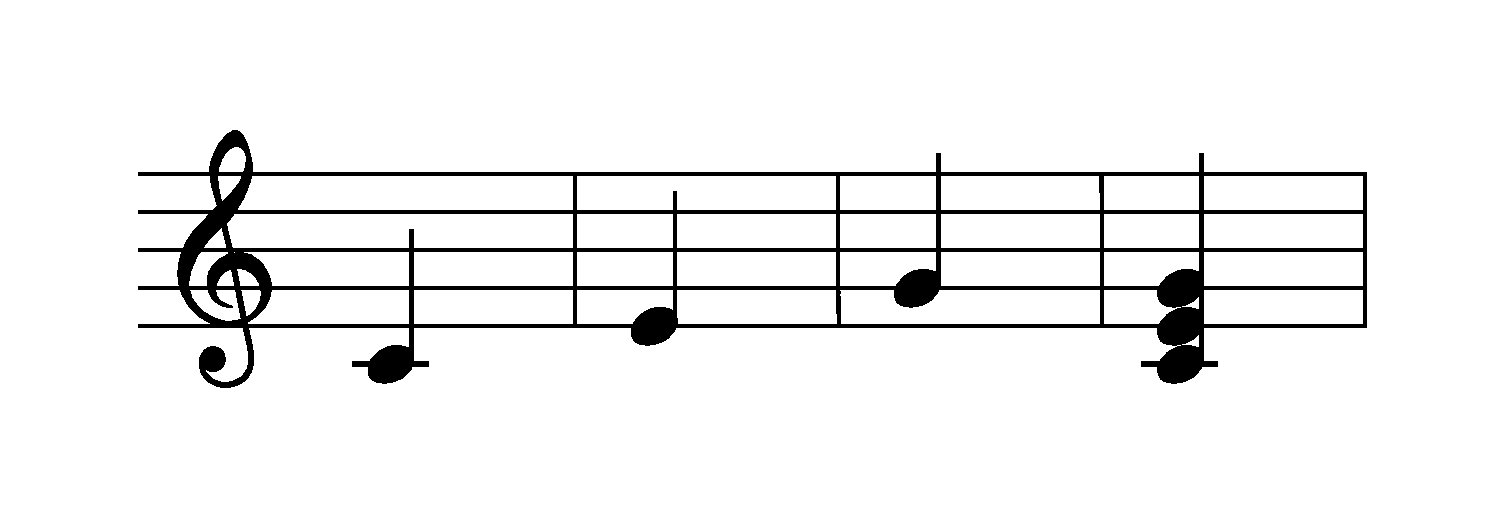
\includegraphics[scale=0.3]{imgs/autoSingleLine}
\end{center}

\columnbreak
all script at once:
\begin{center}
 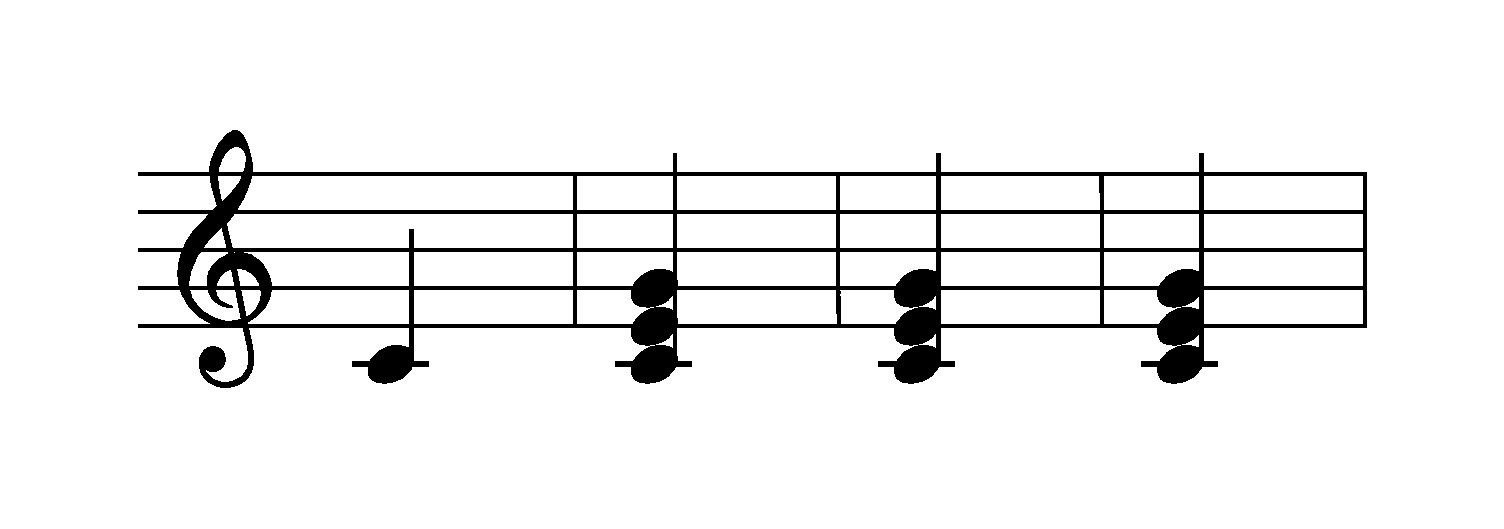
\includegraphics[scale=0.3]{imgs/autoAllScript}
\end{center}

\end{multicols}

To avoid such undeterministic behaviour, one should, in this case, manually trigger \OSC{reeval} after each modification of \OSC{score}.


\printindex

\end{document}
